%%%%%%%%%%%%%%%%%%%%%%%%%%%%%%%%%%%%%%%%%%%%%%%%%%%%%%%%%%%%%%%%%%%%%%
\section{The HTCondorView Client Contrib Module}\label{sec:HTCondorView-Client-Install}
%%%%%%%%%%%%%%%%%%%%%%%%%%%%%%%%%%%%%%%%%%%%%%%%%%%%%%%%%%%%%%%%%%%%%%
\index{HTCondorView!Client}
\index{contrib module!HTCondorView client}

The HTCondorView Client contrib module is used to automatically generate
World Wide Web pages to display usage statistics of an HTCondor
pool.
Included in the module is a shell script which invokes the \Condor{stats}
command to retrieve pool usage statistics from the HTCondorView server, and
generate HTML pages from the results.  
Also included is a Java applet, which graphically visualizes HTCondor 
usage information.  
Users can interact with the applet to customize the visualization and to
zoom in to a specific time frame.
Figure~\ref{fig:view-screenshot} on page~\pageref{fig:view-screenshot}
is a screen shot of a web page created by HTCondorView.  
%  link gone, and script is not working Dec 2012
%To get a further feel for what pages generated by HTCondorView look like,
%view the statistics for the University of Wisconsin-Madison pool 
%by visiting the URL 
%\URL{http://condor-view.cs.wisc.edu/condor-view-applet}.

\begin{figure}[hbt]
\centering
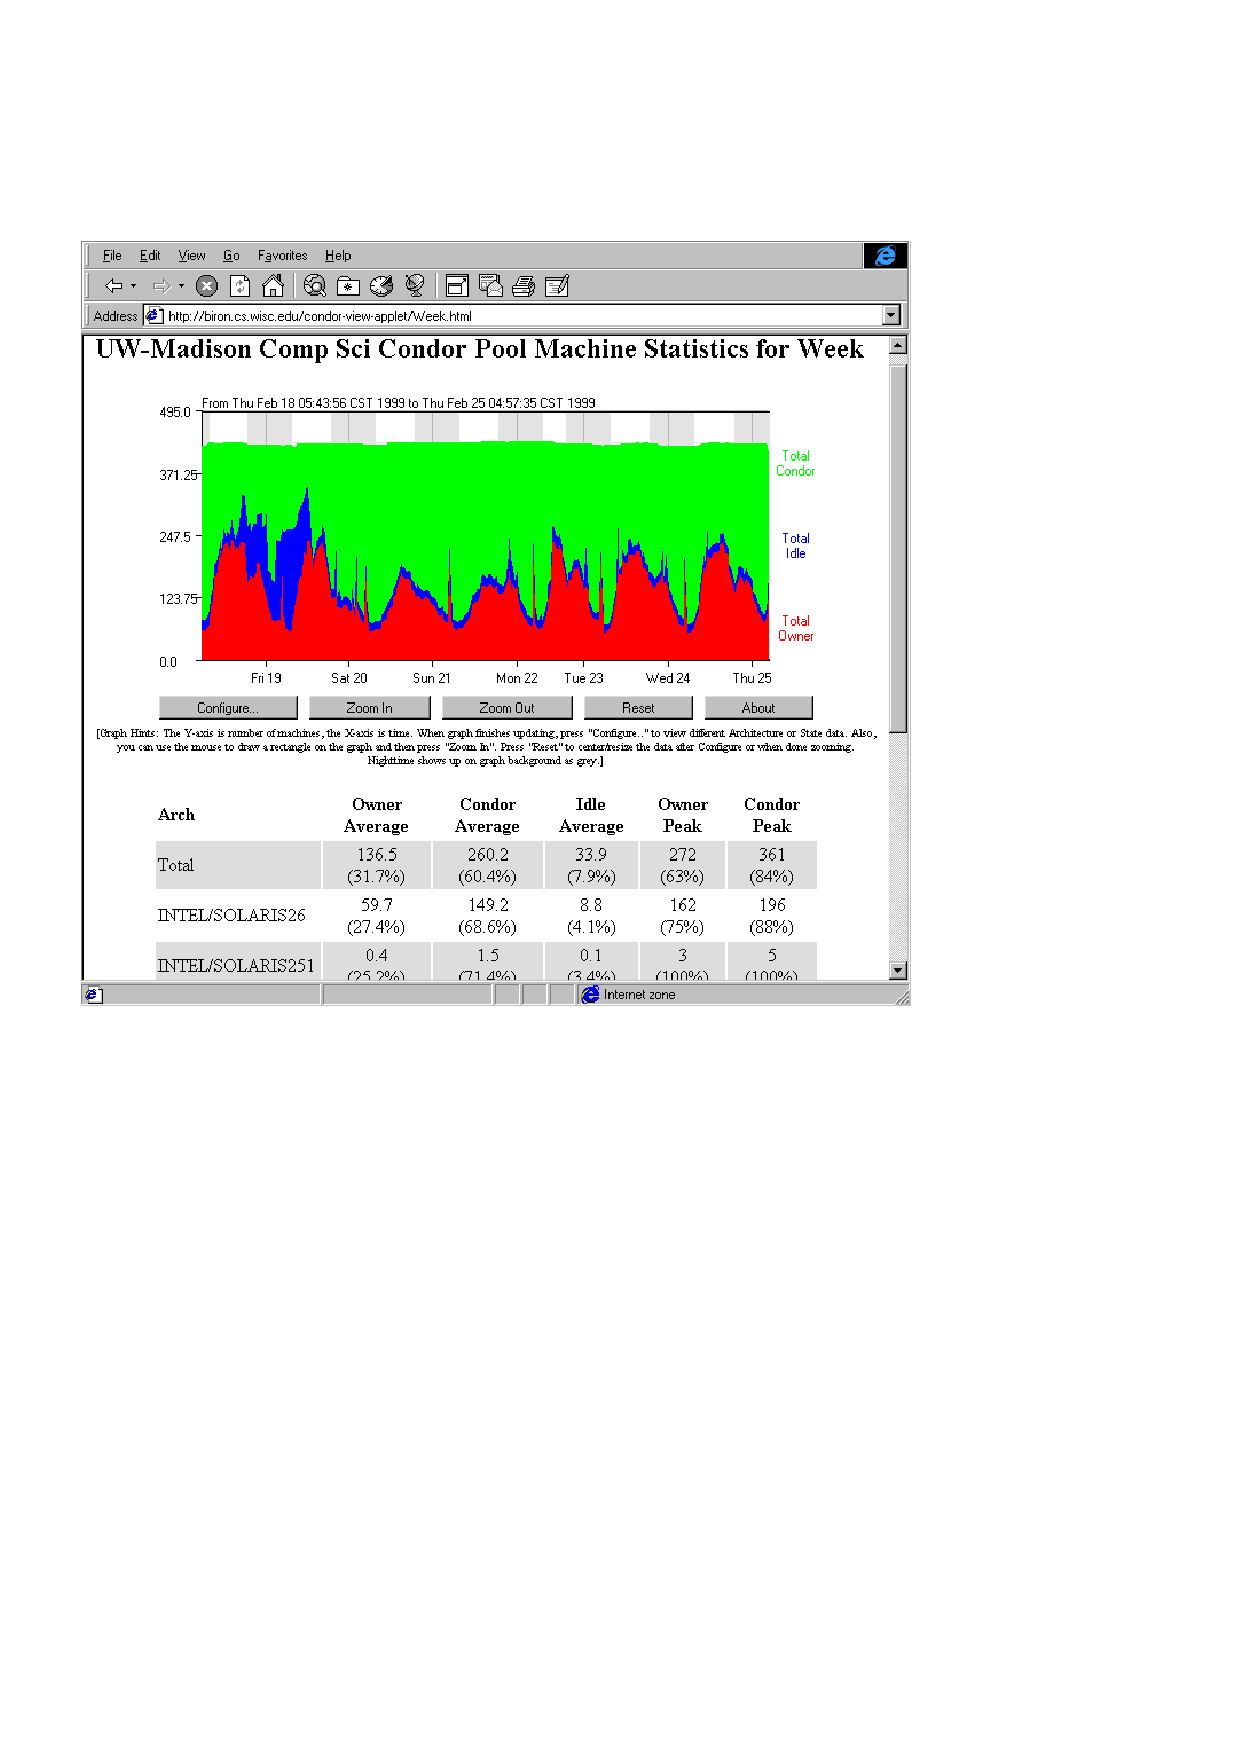
\includegraphics{contrib/view-screenshot}
\caption{\label{fig:view-screenshot}Screen shot of HTCondorView Client}
\end{figure}

After unpacking and installing the HTCondorView Client, a script named
\Prog{make\_stats} can be invoked to create HTML pages displaying HTCondor usage
for the past hour, day, week, or month.  
By using the Unix \Prog{cron} facility to periodically execute
\Prog{make\_stats}, HTCondor pool usage statistics can be kept up to date
automatically.  
This simple model allows the HTCondorView Client to be easily installed;
no Web server CGI interface is needed.

%%%%%%%%%%%%%%%%%%%%%%%%%%%%%%%%%%%%%%%%%%%%%%%%%%%%%%%%%%%%%%%%%%%%%%
\subsection{\label{sec:condorview-client-step-by-step}
Step-by-Step Installation of the HTCondorView Client}
%%%%%%%%%%%%%%%%%%%%%%%%%%%%%%%%%%%%%%%%%%%%%%%%%%%%%%%%%%%%%%%%%%%%%%

\index{installation!HTCondorView Client}
\index{HTCondorView!Client installation}
\begin{enumerate}

\item Make certain that the HTCondorView Server is configured.
Section ~\ref{sec:Contrib-HTCondorView-Install}
describes configuration of the server.
The server logs information on disk in order to provide a persistent,
historical database of pool statistics.
The HTCondorView Client makes queries over the network to this
database.
The \Condor{collector} includes this database support.
To activate the persistent database logging, add the following entries to
the configuration file for the \Condor{collector} chosen to act as the ViewServer.
\begin{verbatim}
    POOL_HISTORY_DIR = /full/path/to/directory/to/store/historical/data 
    KEEP_POOL_HISTORY = True 
\end{verbatim}

\item Create a directory where HTCondorView is to place the HTML files.  
This directory should be one published by a web server, so that HTML
files which exist in this directory can be accessed using a web browser.  
This directory is referred to as the \File{VIEWDIR} directory.

\item Download the \Prog{view\_client} contrib module.
Follow links for contrib modules from the wiki at
\URL{https://htcondor-wiki.cs.wisc.edu/index.cgi/wiki}.

\item Unpack or untar this contrib module into the
directory \File{VIEWDIR}.
This creates several files and subdirectories.
Further unpack the jar file within the \File{VIEWDIR} directory with:
\begin{verbatim} 
  jar -xf condorview.jar
\end{verbatim}

\item Edit the \Prog{make\_stats} script.  At the beginning of the file
are six parameters to customize.
The parameters are

        \begin{description}

	\item[\MacroNI{ORGNAME}] A brief name that identifies an
	organization. An example is ``Univ of Wisconsin''.  Do not
	use any slashes in the name or other special regular-expression
	characters. Avoid the characters \verb@\@ \^\ and \$.

	\item[\MacroNI{CONDORADMIN}] The e-mail
	address of the HTCondor administrator at your site.  
	This e-mail address will appear at the bottom of the web pages.

	\item[\MacroNI{VIEWDIR}] The full path name
	(\emph{not} a relative path) to the \File{VIEWDIR} directory set
	by installation step 2.  
	It is the directory that contains the \Prog{make\_stats} script.

	\item[\MacroNI{STATSDIR}]  The full path name of the
	directory which contains the \Condor{stats} binary.
	The \Condor{stats} program is included in the \Release{bin}
	directory. 
	The value for \MacroNI{STATSDIR} is added to the \MacroNI{PATH}
	parameter by default.  

	\item[\MacroNI{PATH}] A list of subdirectories,
	separated by colons, where the \Prog{make\_stats} script can find
	the \Prog{awk}, \Prog{bc}, \Prog{sed}, \Prog{date}, and \Condor{stats}
	programs.  
	If \Prog{perl} is installed, the path should also
	include the directory where \Prog{perl} is installed.
	The following default works on most systems:
        \begin{verbatim} 
        PATH=/bin:/usr/bin:$STATSDIR:/usr/local/bin
        \end{verbatim}

        \end{description}

\item To create all of the initial HTML files, run
\begin{verbatim}
        ./make_stats setup  
\end{verbatim}
Open the file \File{index.html} to verify that things look good.

\index{HTCondorView!use of \Prog{crontab} program}
\index{crontab program}

\item Add the \Prog{make\_stats} program to \Prog{cron}.  
Running \Prog{make\_stats} in step 6 created a \File{cronentries} file.
This \File{cronentries} file is ready to be processed by the Unix
\Prog{crontab} command.
The \Prog{crontab} manual page contains details about
the \Prog{crontab} command and the \Prog{cron} daemon.
Look at the
\File{cronentries} file; by default, it will run 
\Prog{make\_stats} \Arg{hour} every 15 minutes, 
\Prog{make\_stats} \Arg{day} once an hour, 
\Prog{make\_stats} \Arg{week} twice per day, and 
\Prog{make\_stats} \Arg{month} once per day.
These are reasonable defaults.  
Add these commands to cron on any
system that can access the \MacroNI{VIEWDIR} and
\MacroNI{STATSDIR} directories,
even on a system that does not have HTCondor installed.
The commands do not need to run as root user;
in fact, they should probably not run as root.  These commands can run
as any user that has read/write access to the \File{VIEWDIR} directory.
The command
\begin{verbatim} 
  crontab cronentries
\end{verbatim}
can set the crontab file;
note that this command overwrites the current, existing crontab file with the 
entries from the file \File{cronentries}.

\item Point the web browser at the \File{VIEWDIR} directory
to complete the installation.

\end{enumerate}

